% Options for packages loaded elsewhere
% Options for packages loaded elsewhere
\PassOptionsToPackage{unicode}{hyperref}
\PassOptionsToPackage{hyphens}{url}
\PassOptionsToPackage{dvipsnames,svgnames,x11names}{xcolor}
%
\documentclass[
  letterpaper,
  DIV=11,
  numbers=noendperiod]{scrartcl}
\usepackage{xcolor}
\usepackage{amsmath,amssymb}
\setcounter{secnumdepth}{-\maxdimen} % remove section numbering
\usepackage{iftex}
\ifPDFTeX
  \usepackage[T1]{fontenc}
  \usepackage[utf8]{inputenc}
  \usepackage{textcomp} % provide euro and other symbols
\else % if luatex or xetex
  \usepackage{unicode-math} % this also loads fontspec
  \defaultfontfeatures{Scale=MatchLowercase}
  \defaultfontfeatures[\rmfamily]{Ligatures=TeX,Scale=1}
\fi
\usepackage{lmodern}
\ifPDFTeX\else
  % xetex/luatex font selection
\fi
% Use upquote if available, for straight quotes in verbatim environments
\IfFileExists{upquote.sty}{\usepackage{upquote}}{}
\IfFileExists{microtype.sty}{% use microtype if available
  \usepackage[]{microtype}
  \UseMicrotypeSet[protrusion]{basicmath} % disable protrusion for tt fonts
}{}
\makeatletter
\@ifundefined{KOMAClassName}{% if non-KOMA class
  \IfFileExists{parskip.sty}{%
    \usepackage{parskip}
  }{% else
    \setlength{\parindent}{0pt}
    \setlength{\parskip}{6pt plus 2pt minus 1pt}}
}{% if KOMA class
  \KOMAoptions{parskip=half}}
\makeatother
% Make \paragraph and \subparagraph free-standing
\makeatletter
\ifx\paragraph\undefined\else
  \let\oldparagraph\paragraph
  \renewcommand{\paragraph}{
    \@ifstar
      \xxxParagraphStar
      \xxxParagraphNoStar
  }
  \newcommand{\xxxParagraphStar}[1]{\oldparagraph*{#1}\mbox{}}
  \newcommand{\xxxParagraphNoStar}[1]{\oldparagraph{#1}\mbox{}}
\fi
\ifx\subparagraph\undefined\else
  \let\oldsubparagraph\subparagraph
  \renewcommand{\subparagraph}{
    \@ifstar
      \xxxSubParagraphStar
      \xxxSubParagraphNoStar
  }
  \newcommand{\xxxSubParagraphStar}[1]{\oldsubparagraph*{#1}\mbox{}}
  \newcommand{\xxxSubParagraphNoStar}[1]{\oldsubparagraph{#1}\mbox{}}
\fi
\makeatother


\usepackage{longtable,booktabs,array}
\usepackage{calc} % for calculating minipage widths
% Correct order of tables after \paragraph or \subparagraph
\usepackage{etoolbox}
\makeatletter
\patchcmd\longtable{\par}{\if@noskipsec\mbox{}\fi\par}{}{}
\makeatother
% Allow footnotes in longtable head/foot
\IfFileExists{footnotehyper.sty}{\usepackage{footnotehyper}}{\usepackage{footnote}}
\makesavenoteenv{longtable}
\usepackage{graphicx}
\makeatletter
\newsavebox\pandoc@box
\newcommand*\pandocbounded[1]{% scales image to fit in text height/width
  \sbox\pandoc@box{#1}%
  \Gscale@div\@tempa{\textheight}{\dimexpr\ht\pandoc@box+\dp\pandoc@box\relax}%
  \Gscale@div\@tempb{\linewidth}{\wd\pandoc@box}%
  \ifdim\@tempb\p@<\@tempa\p@\let\@tempa\@tempb\fi% select the smaller of both
  \ifdim\@tempa\p@<\p@\scalebox{\@tempa}{\usebox\pandoc@box}%
  \else\usebox{\pandoc@box}%
  \fi%
}
% Set default figure placement to htbp
\def\fps@figure{htbp}
\makeatother





\setlength{\emergencystretch}{3em} % prevent overfull lines

\providecommand{\tightlist}{%
  \setlength{\itemsep}{0pt}\setlength{\parskip}{0pt}}



 


\KOMAoption{captions}{tableheading}
\makeatletter
\@ifpackageloaded{caption}{}{\usepackage{caption}}
\AtBeginDocument{%
\ifdefined\contentsname
  \renewcommand*\contentsname{Table of contents}
\else
  \newcommand\contentsname{Table of contents}
\fi
\ifdefined\listfigurename
  \renewcommand*\listfigurename{List of Figures}
\else
  \newcommand\listfigurename{List of Figures}
\fi
\ifdefined\listtablename
  \renewcommand*\listtablename{List of Tables}
\else
  \newcommand\listtablename{List of Tables}
\fi
\ifdefined\figurename
  \renewcommand*\figurename{Figure}
\else
  \newcommand\figurename{Figure}
\fi
\ifdefined\tablename
  \renewcommand*\tablename{Table}
\else
  \newcommand\tablename{Table}
\fi
}
\@ifpackageloaded{float}{}{\usepackage{float}}
\floatstyle{ruled}
\@ifundefined{c@chapter}{\newfloat{codelisting}{h}{lop}}{\newfloat{codelisting}{h}{lop}[chapter]}
\floatname{codelisting}{Listing}
\newcommand*\listoflistings{\listof{codelisting}{List of Listings}}
\makeatother
\makeatletter
\makeatother
\makeatletter
\@ifpackageloaded{caption}{}{\usepackage{caption}}
\@ifpackageloaded{subcaption}{}{\usepackage{subcaption}}
\makeatother
\usepackage{bookmark}
\IfFileExists{xurl.sty}{\usepackage{xurl}}{} % add URL line breaks if available
\urlstyle{same}
\hypersetup{
  pdftitle={Predicting Post-Graduation Earnings},
  pdfauthor={Ava Lasater},
  colorlinks=true,
  linkcolor={blue},
  filecolor={Maroon},
  citecolor={Blue},
  urlcolor={Blue},
  pdfcreator={LaTeX via pandoc}}


\title{Predicting Post-Graduation Earnings}
\usepackage{etoolbox}
\makeatletter
\providecommand{\subtitle}[1]{% add subtitle to \maketitle
  \apptocmd{\@title}{\par {\large #1 \par}}{}{}
}
\makeatother
\subtitle{INFO 523 - Fall 2025 - Final Project}
\author{Ava Lasater}
\date{}
\begin{document}
\maketitle


\subsection{Overview}\label{overview}

\begin{itemize}
\tightlist
\item
  \textbf{Goal:} Understand how tuition, financial burden, and
  institutional characteristics relate to post-graduation earnings.
\item
  \textbf{Data:} U.S. Department of Education \textbf{College Scorecard}
\item
  \textbf{Methods:}

  \begin{itemize}
  \tightlist
  \item
    Exploratory data analysis
  \item
    Linear \& Ridge regression
  \item
    Logistic regression \& Random Forest
  \item
    Feature selection \& permutation importance
  \end{itemize}
\item
  \textbf{Key focus:} Which institutional features most strongly predict
  higher earnings 10 years after enrollment?
\end{itemize}

\begin{center}\rule{0.5\linewidth}{0.5pt}\end{center}

\subsection{Research Questions}\label{research-questions}

\begin{itemize}
\tightlist
\item
  \textbf{RQ1.} How do tuition and financial burden relate to median
  earnings 10 years after enrollment?
\item
  \textbf{RQ2.} How do institutional characteristics (region, locale,
  control, size) and student composition (Pell share) relate to earnings
  and completion?
\item
  \textbf{RQ3.} Can institutional features reliably classify colleges as
  \textbf{high-earning vs.~low-earning}?
\item
  \textbf{RQ4.} Which features are most important for prediction across
  linear and machine-learning models?
\end{itemize}

\begin{center}\rule{0.5\linewidth}{0.5pt}\end{center}

\subsection{Data \& Preprocessing}\label{data-preprocessing}

\begin{itemize}
\tightlist
\item
  \textbf{Source:} U.S. College Scorecard (institution-level data).
\item
  \textbf{Scope:}

  \begin{itemize}
  \tightlist
  \item
    Filtered to institutions that \textbf{primarily award bachelor's
    degrees}.
  \item
    Focused on recent cohorts with available 10-year earnings.
  \end{itemize}
\item
  \textbf{Key variable groups:}

  \begin{itemize}
  \tightlist
  \item
    \textbf{Cost:} in-state \& out-of-state tuition, median debt.
  \item
    \textbf{Institutional:} enrollment (UGDS), control, region, locale.
  \item
    \textbf{Outcomes:} retention, 4-year completion, 10-year median
    earnings.
  \end{itemize}
\item
  \textbf{Missing data:}

  \begin{itemize}
  \tightlist
  \item
    Dropped columns with severe missingness (e.g., detailed
    demographics).
  \item
    Dropped rows with missing core cost/outcome variables rather than
    imputing.
  \end{itemize}
\end{itemize}

\begin{center}\rule{0.5\linewidth}{0.5pt}\end{center}

\subsection{Sample Structure Check}\label{sample-structure-check}

\begin{itemize}
\tightlist
\item
  Compared \textbf{original vs.~cleaned} distributions for:

  \begin{itemize}
  \tightlist
  \item
    State, region, locale, and control type.
  \end{itemize}
\item
  \textbf{Result:} Filtering and missing-data removal:

  \begin{itemize}
  \tightlist
  \item
    Did \textbf{not} wipe out any region or control group.
  \item
    Preserved a broad mix of public and private institutions across the
    U.S.
  \end{itemize}
\item
  Interpretation: The cleaned dataset still represents a diverse
  institutional landscape.
\end{itemize}

\begin{center}\rule{0.5\linewidth}{0.5pt}\end{center}

\subsection{Distribution of Institutions by
Region}\label{distribution-of-institutions-by-region}

\begin{center}
\pandocbounded{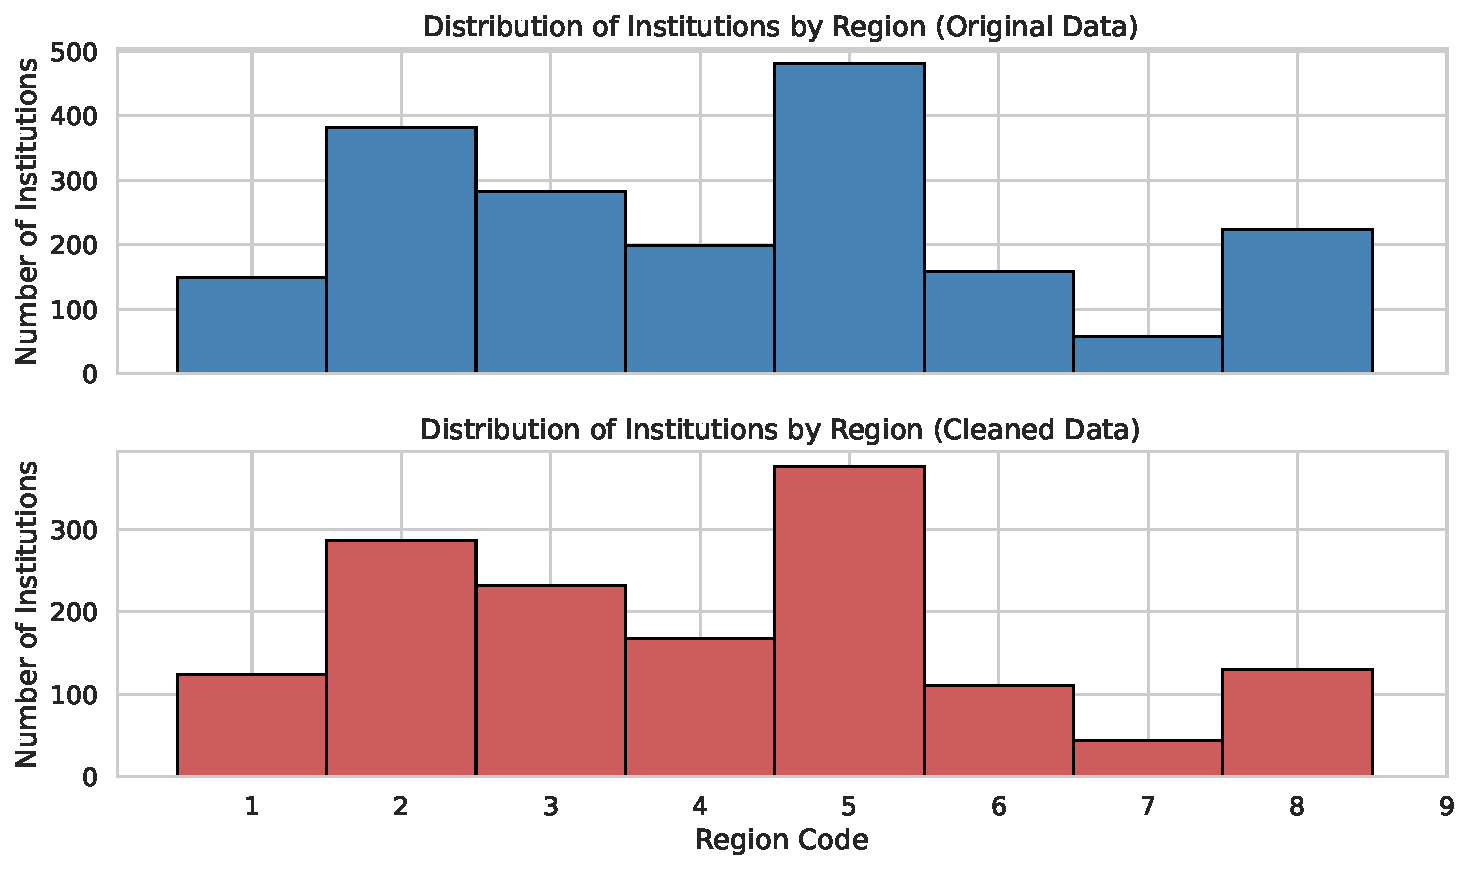
\includegraphics[keepaspectratio]{presentation_files/figure-pdf/cell-5-output-1.pdf}}
\end{center}

\begin{center}\rule{0.5\linewidth}{0.5pt}\end{center}

\subsection{Distribution of Institutions by
Locale}\label{distribution-of-institutions-by-locale}

\begin{center}
\pandocbounded{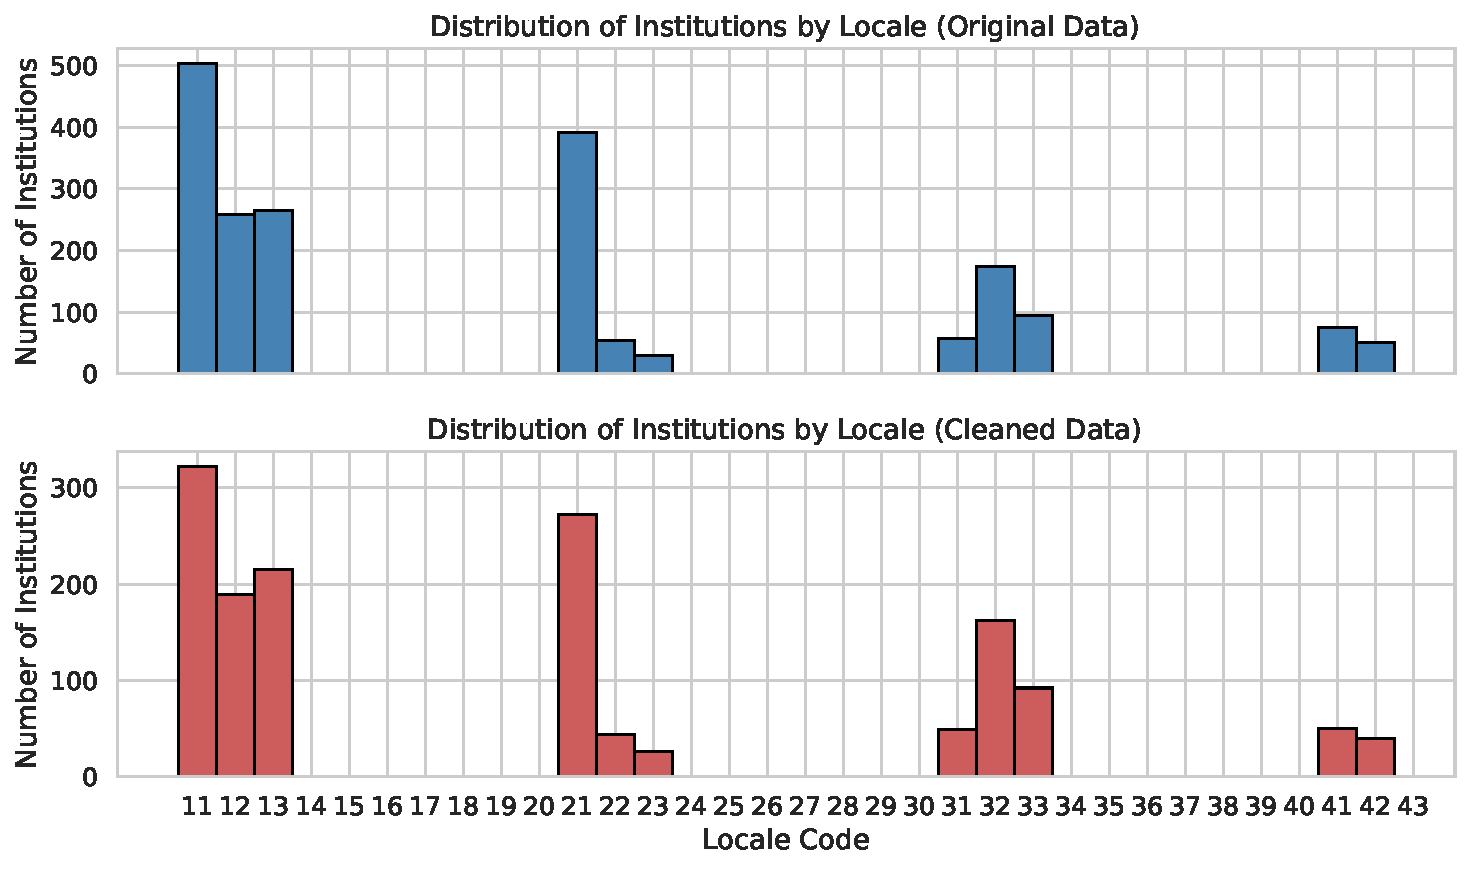
\includegraphics[keepaspectratio]{presentation_files/figure-pdf/cell-6-output-1.pdf}}
\end{center}

\begin{center}\rule{0.5\linewidth}{0.5pt}\end{center}

\subsection{Distribution of Institutions by
Control}\label{distribution-of-institutions-by-control}

\begin{center}
\pandocbounded{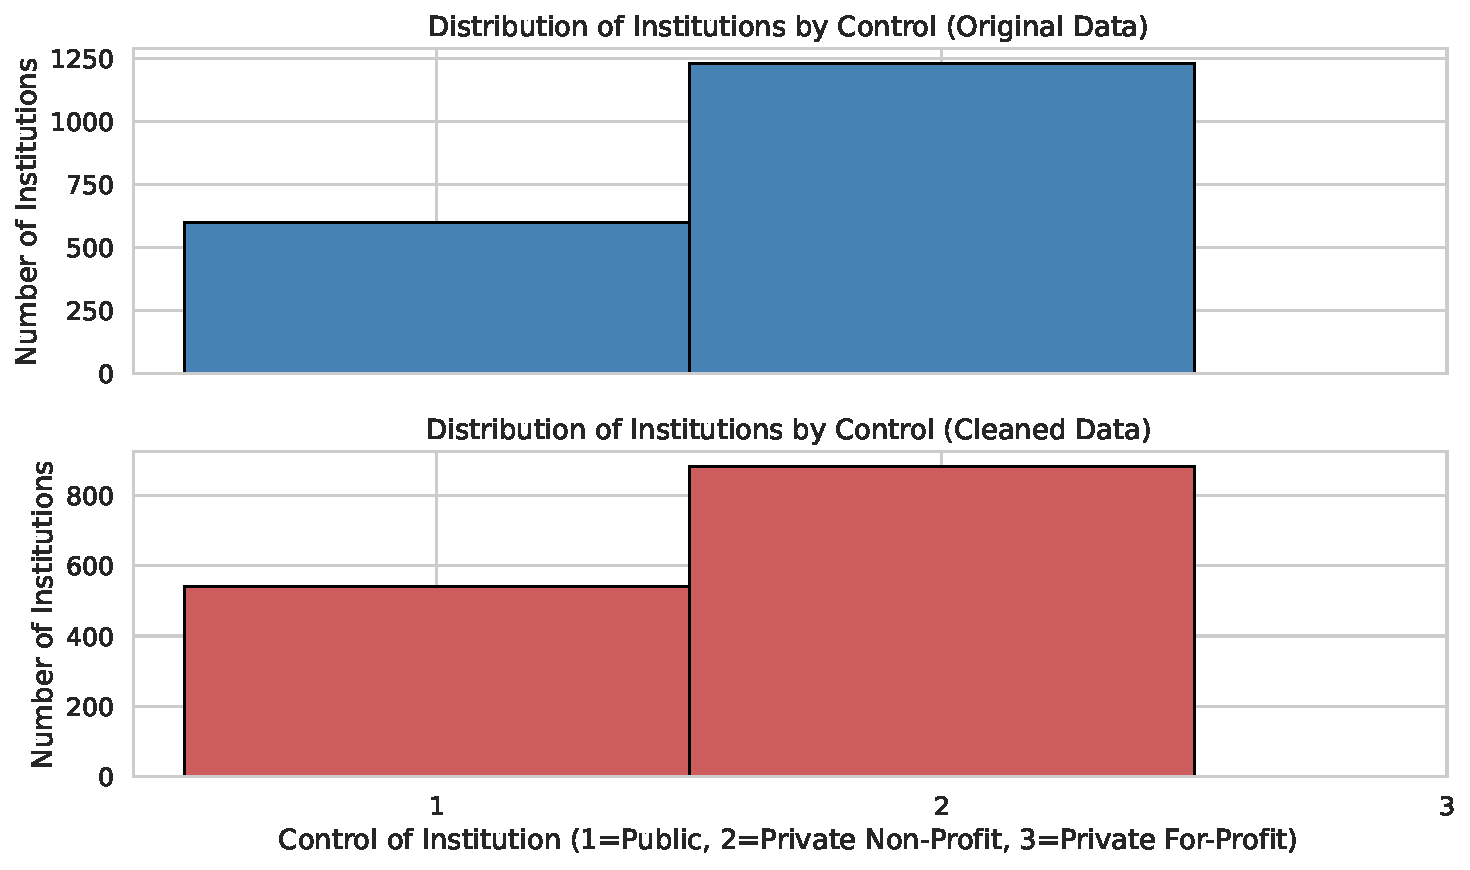
\includegraphics[keepaspectratio]{presentation_files/figure-pdf/cell-7-output-1.pdf}}
\end{center}

\begin{center}\rule{0.5\linewidth}{0.5pt}\end{center}

\subsection{Exploratory Data Analysis}\label{exploratory-data-analysis}

\begin{itemize}
\tightlist
\item
  \textbf{Cost:}

  \begin{itemize}
  \tightlist
  \item
    In-state and out-of-state tuition are \textbf{right-skewed}.
  \item
    Most schools between ≈ \$10K--\$40K; a small number of very
    expensive institutions.
  \end{itemize}
\item
  \textbf{Size (UGDS):}

  \begin{itemize}
  \tightlist
  \item
    Strong right skew; most enroll 1K--6K students.
  \item
    A few very large institutions (e.g., large online providers).
  \end{itemize}
\item
  \textbf{Outcomes:}

  \begin{itemize}
  \tightlist
  \item
    Retention and completion rates are bounded {[}0,1{]} and cluster
    toward higher values.
  \item
    Identified and removed institutions with impossible patterns (e.g.,
    0\% completion at all time horizons, 0\% retention with missing
    context).
  \end{itemize}
\item
  \textbf{Earnings:}

  \begin{itemize}
  \tightlist
  \item
    10-year earnings percentiles are skewed; \textbf{median earnings}
    used as a stable target.
  \end{itemize}
\end{itemize}

\begin{center}\rule{0.5\linewidth}{0.5pt}\end{center}

\subsection{Correlation Patterns}\label{correlation-patterns}

\begin{itemize}
\tightlist
\item
  Tuition has \textbf{only weak to moderate correlation} with earnings.
\item
  Retention and completion rates show \textbf{moderate positive}
  correlations with earnings.
\item
  Pell Grant share (\textbf{PCTPELL}) shows \textbf{negative}
  correlations with both earnings and completion:

  \begin{itemize}
  \tightlist
  \item
    Institutions serving more low-income students tend to have lower
    median earnings.
  \end{itemize}
\item
  Takeaway: \textbf{Institutional performance and student composition}
  are more strongly related to outcomes than tuition alone.
\end{itemize}

\begin{center}\rule{0.5\linewidth}{0.5pt}\end{center}

\subsection{Correlation Matrix of Numerical
Features}\label{correlation-matrix-of-numerical-features}

\begin{center}
\pandocbounded{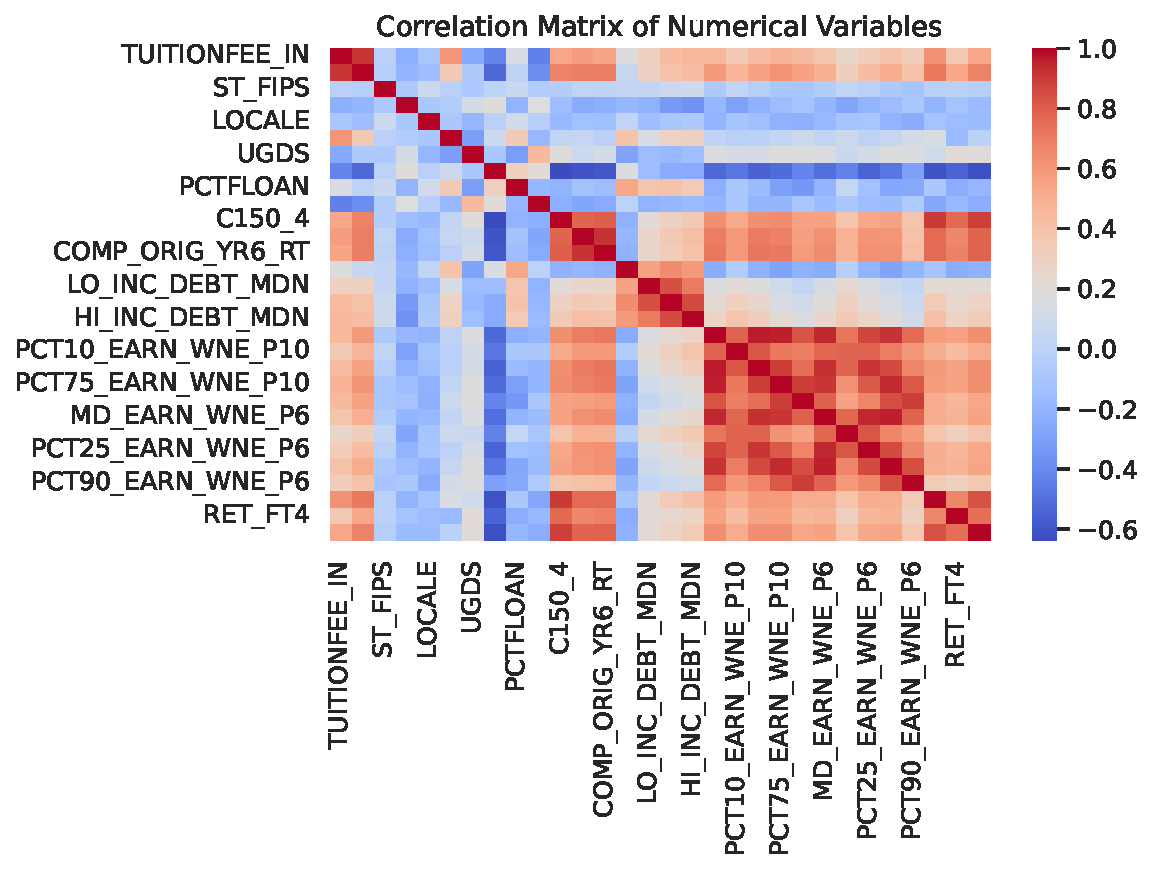
\includegraphics[keepaspectratio]{presentation_files/figure-pdf/cell-8-output-1.pdf}}
\end{center}

\begin{center}\rule{0.5\linewidth}{0.5pt}\end{center}

\subsection{Regression Setup}\label{regression-setup}

\begin{itemize}
\tightlist
\item
  \textbf{Target:} Median earnings 10 years after enrollment
  (\textbf{MD\_EARN\_WNE\_P10}).
\item
  \textbf{Predictors:}

  \begin{itemize}
  \tightlist
  \item
    Cost: TUITIONFEE\_IN, TUITIONFEE\_OUT, median debt.
  \item
    Institution: UGDS, region dummies, locale dummies, control dummies.
  \item
    Outcomes: retention and completion rates.
  \end{itemize}
\item
  \textbf{Preprocessing:}

  \begin{itemize}
  \tightlist
  \item
    Log-transform skewed variables where appropriate.
  \item
    Standardize continuous predictors.
  \item
    One-hot encode categorical variables (region, locale, control).
  \end{itemize}
\end{itemize}

\begin{center}\rule{0.5\linewidth}{0.5pt}\end{center}

\subsection{Linear \& Ridge Regression
Results}\label{linear-ridge-regression-results}

\begin{itemize}
\tightlist
\item
  \textbf{Linear model (OLS):}

  \begin{itemize}
  \tightlist
  \item
    Adjusted R² ≈ 0.57 --- institutional features explain over half of
    the variation in 10-year earnings.
  \item
    Largest positive coefficients: in-state tuition, first-year
    retention, 4-year completion, and enrollment size.
  \item
    Largest negative coefficients: Pell Grant share (PCTPELL), median
    student debt, and several lower-earning regional indicators.
  \end{itemize}
\item
  \textbf{Multicollinearity:}

  \begin{itemize}
  \tightlist
  \item
    High VIF for tuition variables → removed out-of-state tuition for
    OLS.
  \item
    Ridge regression refit with both tuition variables:

    \begin{itemize}
    \tightlist
    \item
      Similar R² (\textasciitilde0.49 on test data).
    \item
      Coefficient plot shows the larget positive effects for
      TUITIONFEE\_IN, RET\_FT4, C100\_4, (completion), TUITIONFEE\_OUT,
      and UGDS (enrollment size).
    \item
      The largest negative effects come from PCTPELL and indicators for
      certain regions (e.g., outlying areas, Rocky Mountains,
      Southeast).
    \end{itemize}
  \end{itemize}
\item
  \textbf{Limitations:}

  \begin{itemize}
  \tightlist
  \item
    Residuals show curvature, heteroscedasticity, and heavy tails →
    linear model is an approximation.
  \end{itemize}
\end{itemize}

\begin{center}\rule{0.5\linewidth}{0.5pt}\end{center}

\subsection{Linear Regression Results}\label{linear-regression-results}

\begin{verbatim}
Mean Squared Error: 110300510.89
R-squared: 0.4855
\end{verbatim}

\begin{center}
\pandocbounded{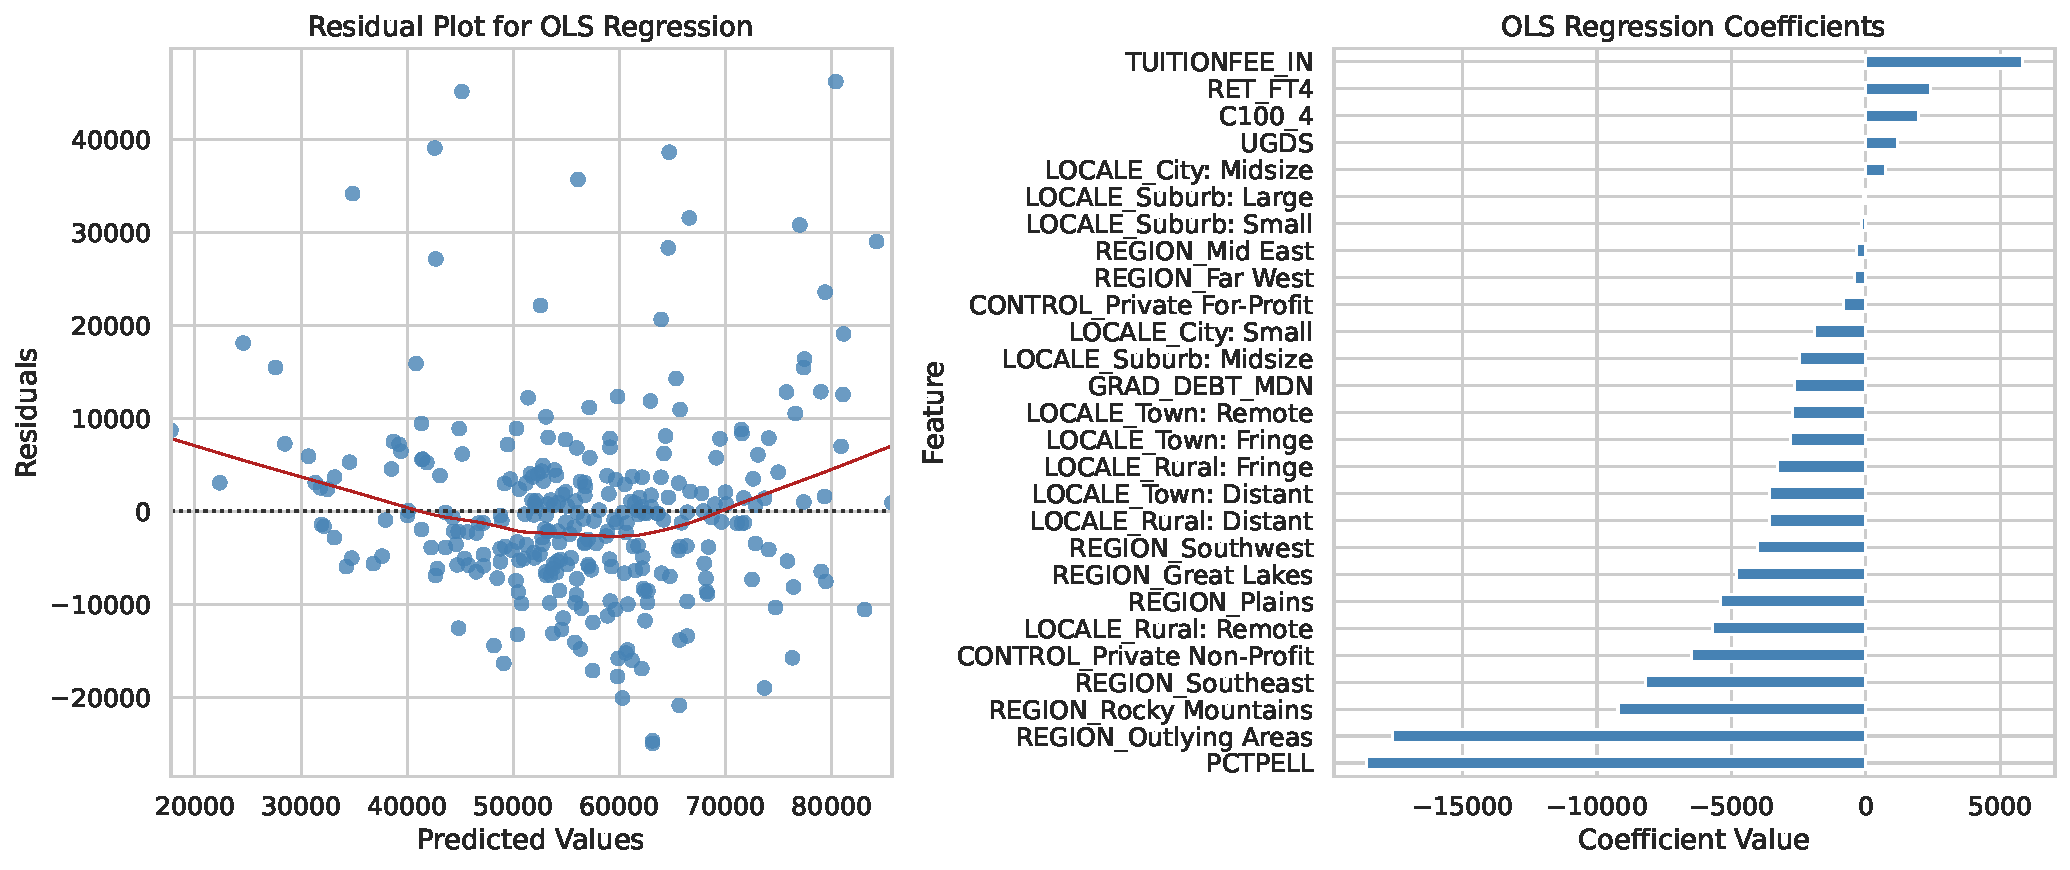
\includegraphics[keepaspectratio]{presentation_files/figure-pdf/cell-9-output-2.pdf}}
\end{center}

\begin{center}\rule{0.5\linewidth}{0.5pt}\end{center}

\subsection{Ridge Regression Results}\label{ridge-regression-results}

\begin{verbatim}
Ridge Regression:
Mean Squared Error: 110226157.793066
R-squared: 0.48583010161522244
\end{verbatim}

\begin{center}
\pandocbounded{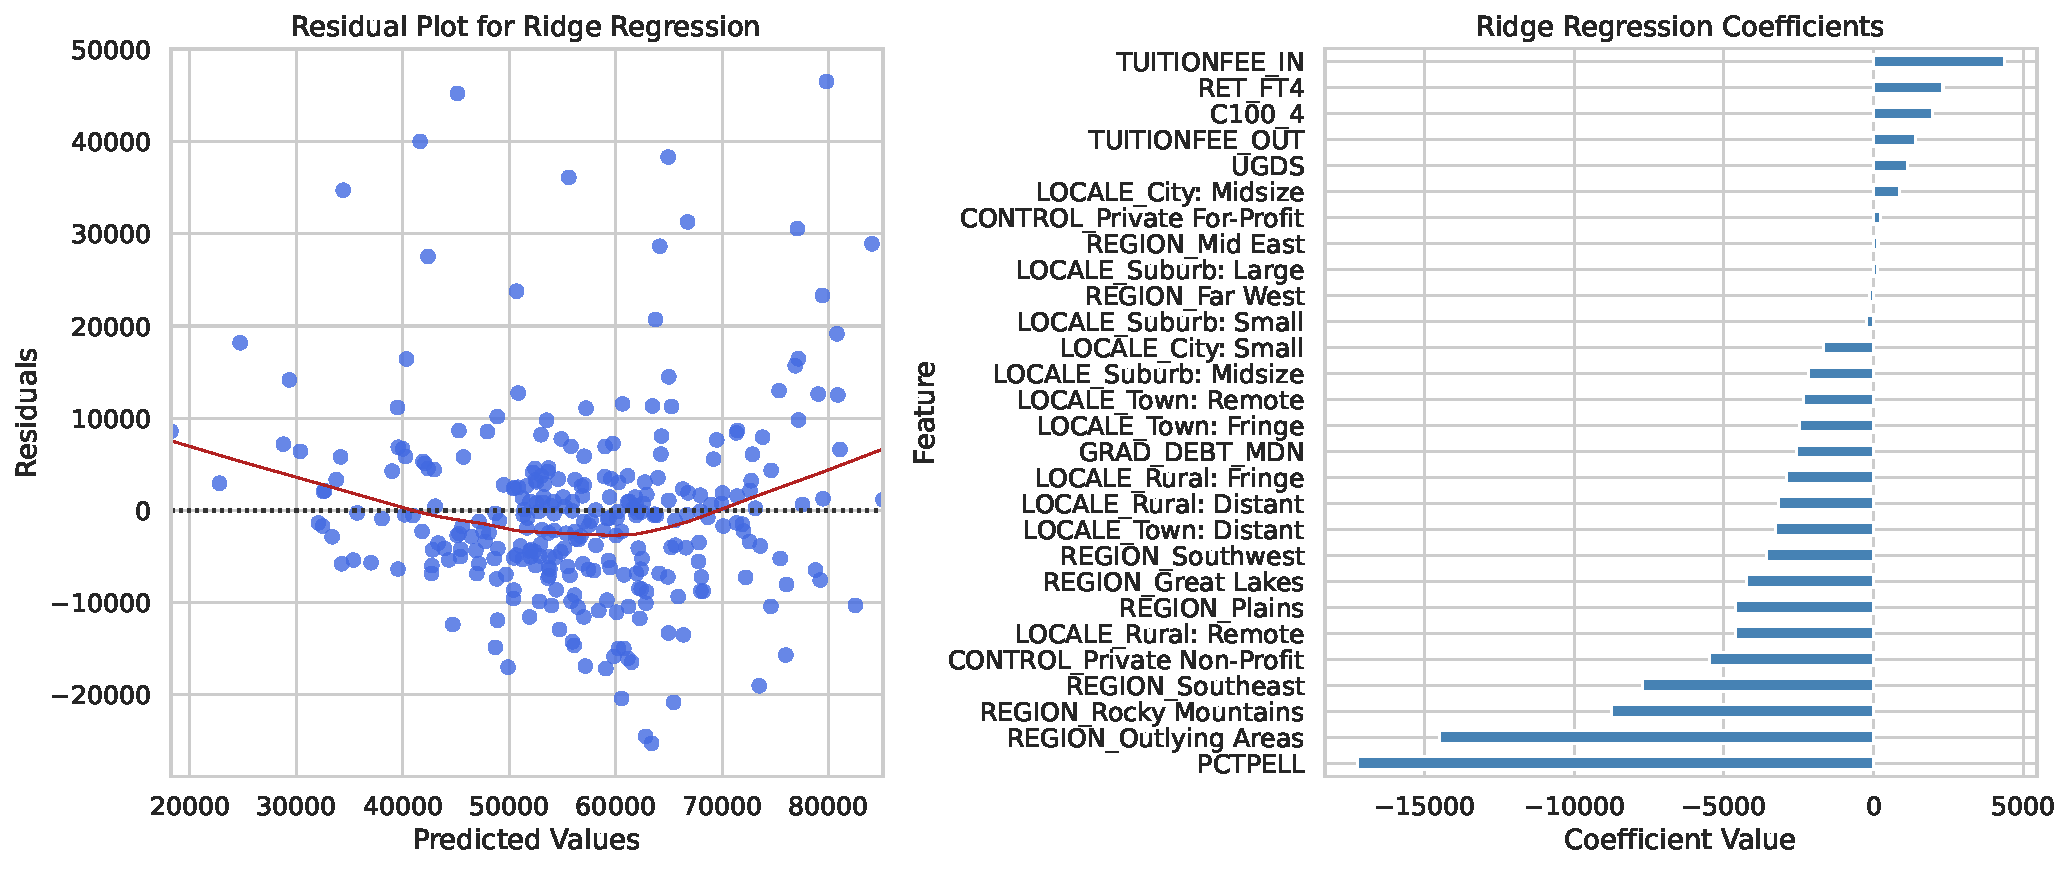
\includegraphics[keepaspectratio]{presentation_files/figure-pdf/cell-10-output-2.pdf}}
\end{center}

\begin{center}\rule{0.5\linewidth}{0.5pt}\end{center}

\subsection{Feature Selection for
Classification}\label{feature-selection-for-classification}

\begin{itemize}
\tightlist
\item
  \textbf{Outcome for classification:} High-earning vs.~low-earning
  institution\\
  (above vs.~below sample median earnings).
\item
  \textbf{Feature selection strategy:}

  \begin{itemize}
  \tightlist
  \item
    \textbf{SelectKBest} (f\_classif) to identify top 15 statistically
    relevant predictors.
  \item
    \textbf{Random Forest feature importance} to capture nonlinear
    effects and interactions.
  \item
    Final feature set = \textbf{union} of the top features from both
    methods.
  \end{itemize}
\item
  \textbf{Self-taught component:}

  \begin{itemize}
  \tightlist
  \item
    Added \textbf{permutation importance} to quantify how much model
    performance drops when each feature is shuffled.
  \end{itemize}
\end{itemize}

\begin{center}\rule{0.5\linewidth}{0.5pt}\end{center}

\subsection{SelectKBest Feature
Selection}\label{selectkbest-feature-selection}

\begin{center}
\pandocbounded{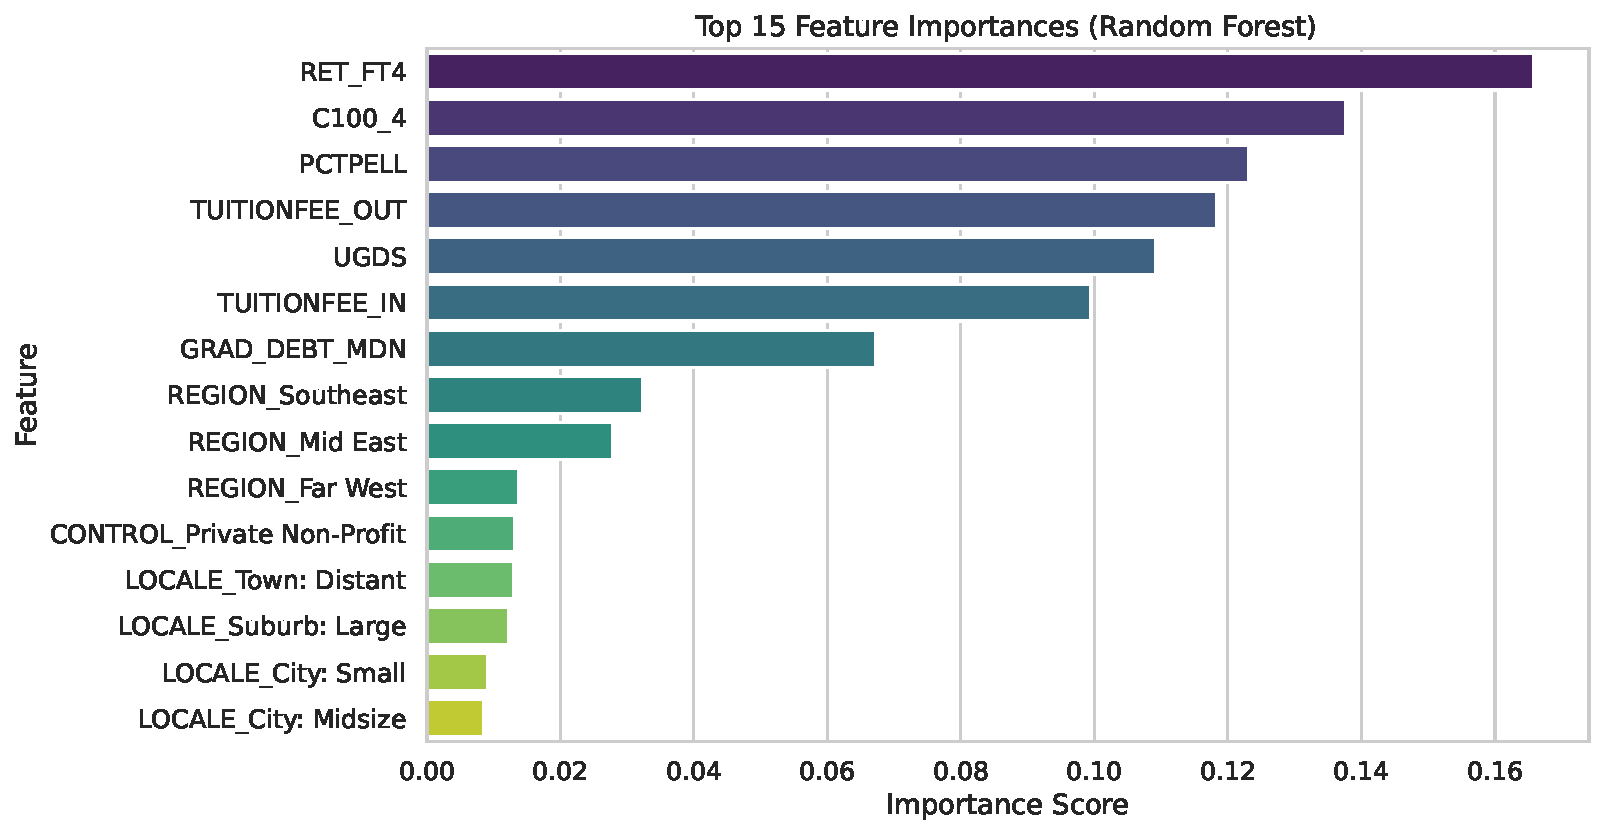
\includegraphics[keepaspectratio]{presentation_files/figure-pdf/cell-11-output-1.pdf}}
\end{center}

\begin{center}\rule{0.5\linewidth}{0.5pt}\end{center}

\subsection{Logistic Regression
Classification}\label{logistic-regression-classification}

\begin{itemize}
\tightlist
\item
  \textbf{Model:} Logistic regression with standardized predictors.
\item
  \textbf{Performance:}

  \begin{itemize}
  \tightlist
  \item
    Accuracy ≈ \textbf{0.77}
  \item
    Precision ≈ \textbf{0.78}
  \item
    Recall ≈ \textbf{0.77}
  \item
    F1 ≈ \textbf{0.77}
  \item
    5-fold CV F1 ≈ \textbf{0.80}
  \end{itemize}
\item
  \textbf{Interpretation:}

  \begin{itemize}
  \tightlist
  \item
    A simple linear decision boundary separates high- and low-earning
    institutions reasonably well.
  \item
    Coefficient patterns mirror regression results: retention,
    completion, tuition, and Pell share are key drivers.
  \end{itemize}
\end{itemize}

\begin{center}\rule{0.5\linewidth}{0.5pt}\end{center}

\subsection{Logistic Regression
Results}\label{logistic-regression-results}

\begin{verbatim}
k-Fold F1-Score: 0.80
k-Fold CV took 0.08 seconds

Logistic Regression Accuracy: 0.7728813559322034
Logistic Regression Precision: 0.7775823831391786
Logisitc Regression Recall: 0.7728813559322034
Logistic Regression F-1 Score: 0.7719854657317307
\end{verbatim}

\begin{center}
\pandocbounded{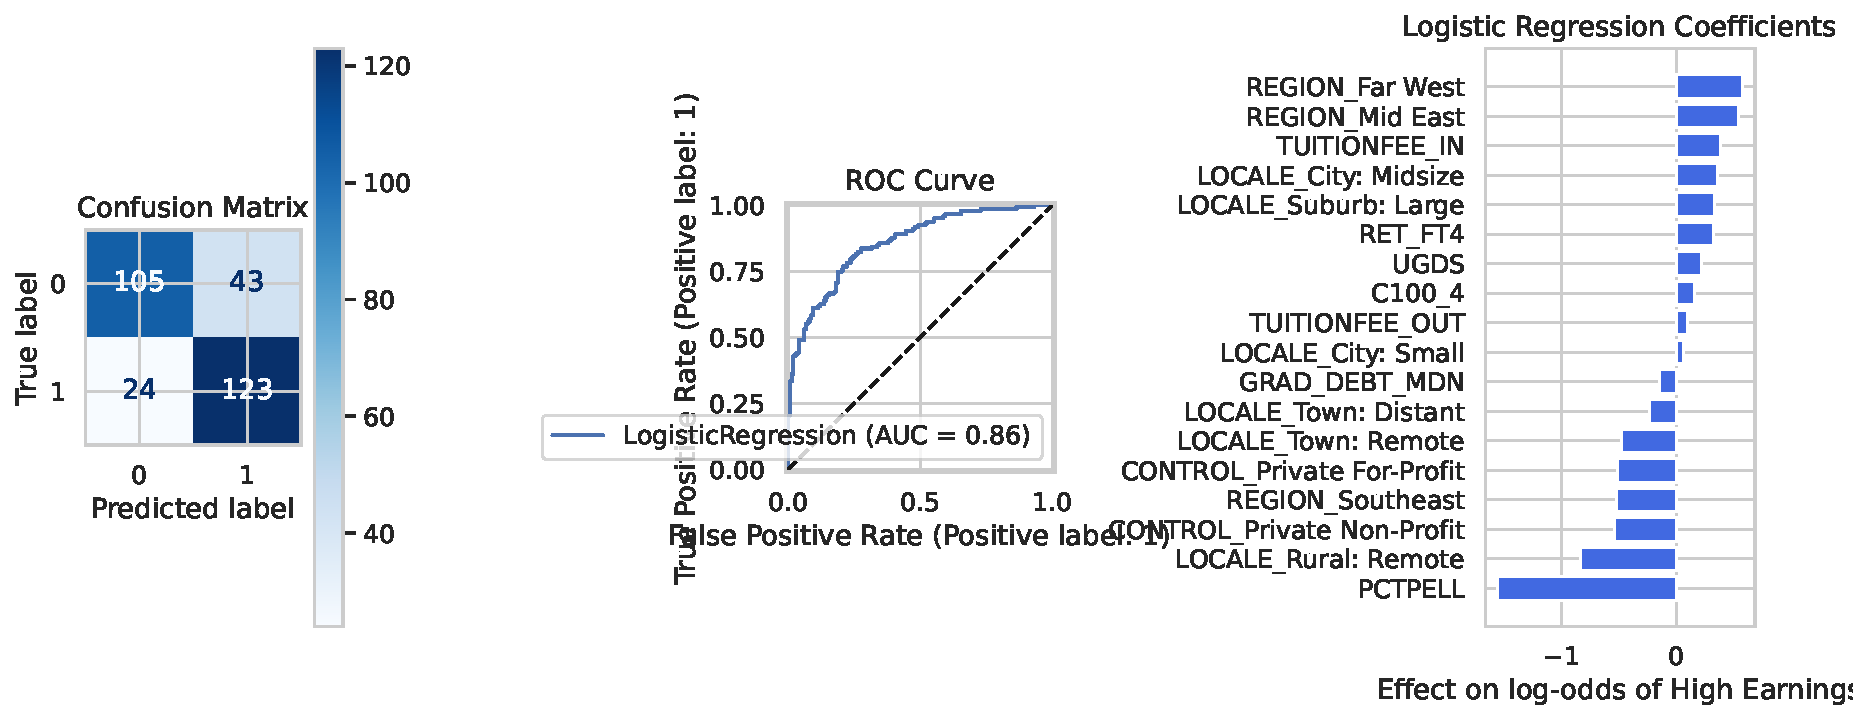
\includegraphics[keepaspectratio]{presentation_files/figure-pdf/cell-12-output-2.pdf}}
\end{center}

\begin{center}\rule{0.5\linewidth}{0.5pt}\end{center}

\subsection{Random Forest
Classification}\label{random-forest-classification}

\begin{itemize}
\tightlist
\item
  \textbf{Model:} Random Forest classifier using the selected feature
  set.
\item
  \textbf{Performance:}

  \begin{itemize}
  \tightlist
  \item
    Accuracy ≈ \textbf{0.78}
  \item
    Precision, Recall, F1 ≈ \textbf{0.78}
  \item
    5-fold CV F1 ≈ \textbf{0.82}
  \end{itemize}
\item
  \textbf{Insights:}

  \begin{itemize}
  \tightlist
  \item
    Slightly better predictive performance than logistic regression.
  \item
    Captures nonlinear relationships and interactions among:

    \begin{itemize}
    \tightlist
    \item
      Enrollment size (UGDS)
    \item
      Retention and completion
    \item
      Tuition levels
    \item
      Pell share
    \item
      Certain regions
    \end{itemize}
  \end{itemize}
\end{itemize}

\begin{center}\rule{0.5\linewidth}{0.5pt}\end{center}

\subsection{Random Forest Results}\label{random-forest-results}

\begin{verbatim}
Random Forest Cross Validation
k-Fold F1-Score: 0.81
k-Fold CV took 1.08 seconds
Random Forest Accuracy: 0.7796610169491526
Random Forest Precision: 0.7819154111738857
Random Forest Recall: 0.7796610169491526
Random Forest F-1 Score: 0.7792653852073915
\end{verbatim}

\begin{center}
\pandocbounded{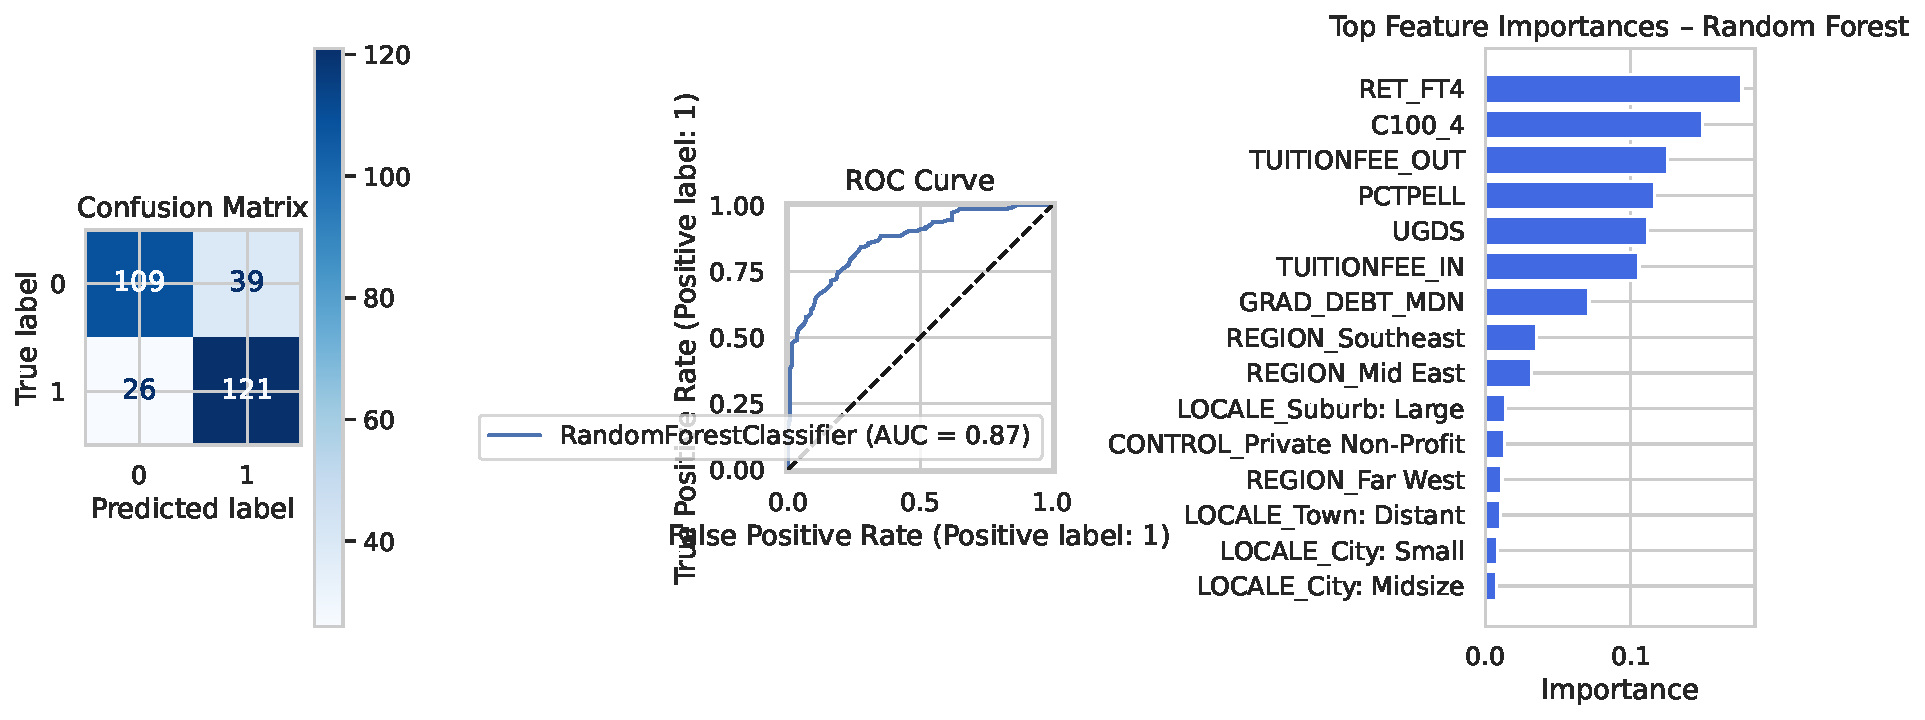
\includegraphics[keepaspectratio]{presentation_files/figure-pdf/cell-13-output-2.pdf}}
\end{center}

\begin{center}\rule{0.5\linewidth}{0.5pt}\end{center}

\subsection{Permutation Importance (Random
Forest)}\label{permutation-importance-random-forest}

\begin{itemize}
\tightlist
\item
  \textbf{Top predictors for high-earning institutions:}

  \begin{itemize}
  \tightlist
  \item
    \textbf{UGDS} (student body size)
  \item
    \textbf{RET\_FT4} (first-year retention)
  \item
    \textbf{TUITIONFEE\_OUT} and \textbf{TUITIONFEE\_IN}
  \item
    \textbf{PCTPELL} (share of Pell recipients)
  \item
    Regional indicators (e.g., Southeast, Mid East)
  \end{itemize}
\item
  \textbf{Low-impact features:}

  \begin{itemize}
  \tightlist
  \item
    Many fine-grained locale categories
  \item
    Control type contributes relatively little once other factors are
    included.
  \end{itemize}
\item
  \textbf{Takeaway:} Structural and academic characteristics (size,
  retention, completion) and student composition matter more than
  geographic setting.
\end{itemize}

\begin{center}\rule{0.5\linewidth}{0.5pt}\end{center}

\subsection{Permutation Importance}\label{permutation-importance}

\begin{center}
\pandocbounded{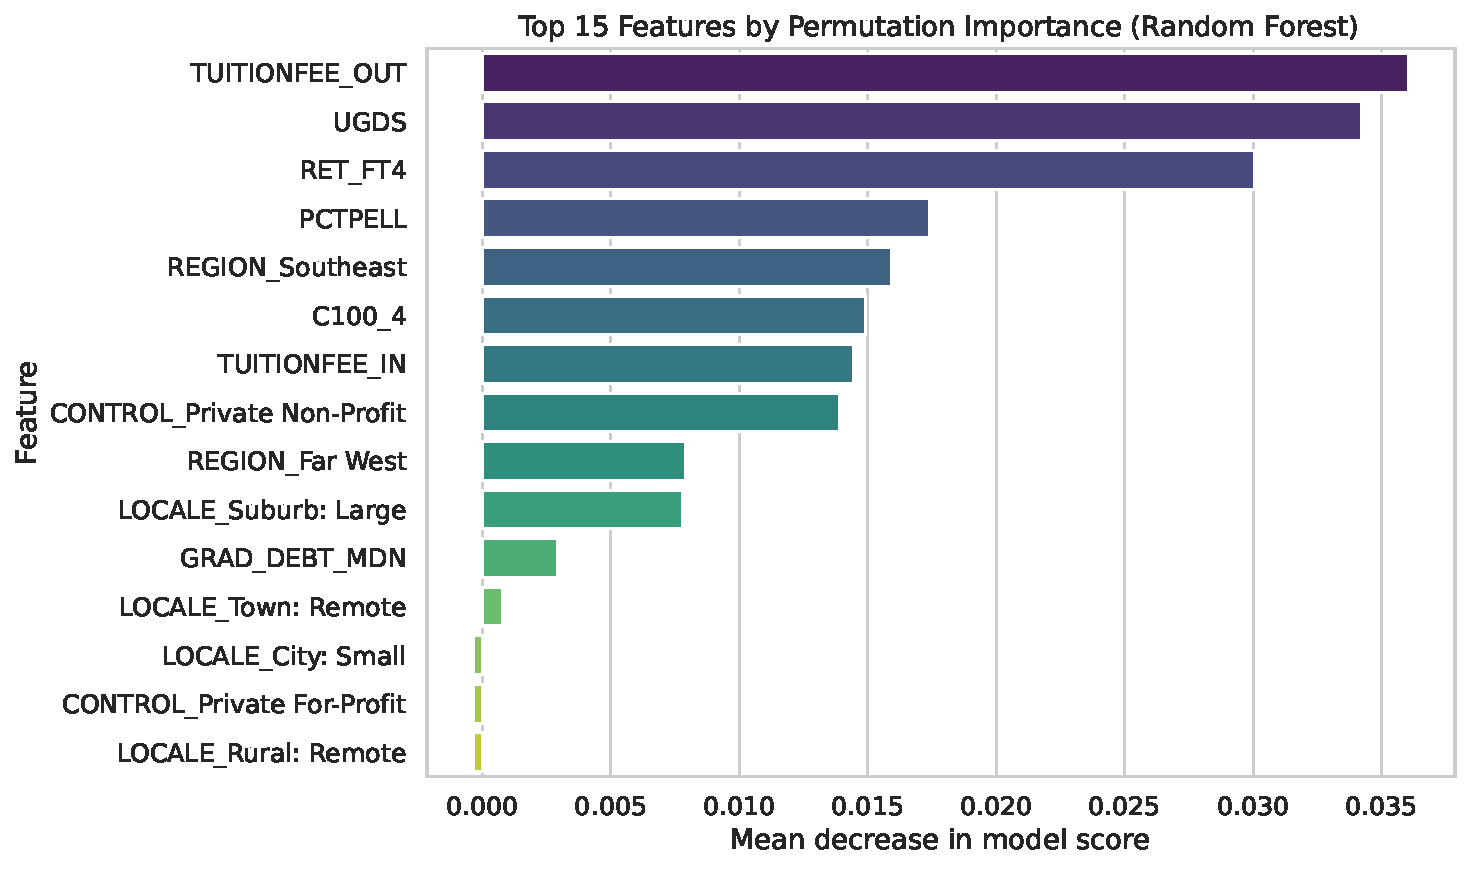
\includegraphics[keepaspectratio]{presentation_files/figure-pdf/cell-14-output-1.pdf}}
\end{center}

\begin{center}\rule{0.5\linewidth}{0.5pt}\end{center}

\subsection{Calibration: Probabilities
vs.~Accuracy}\label{calibration-probabilities-vs.-accuracy}

\begin{center}
\pandocbounded{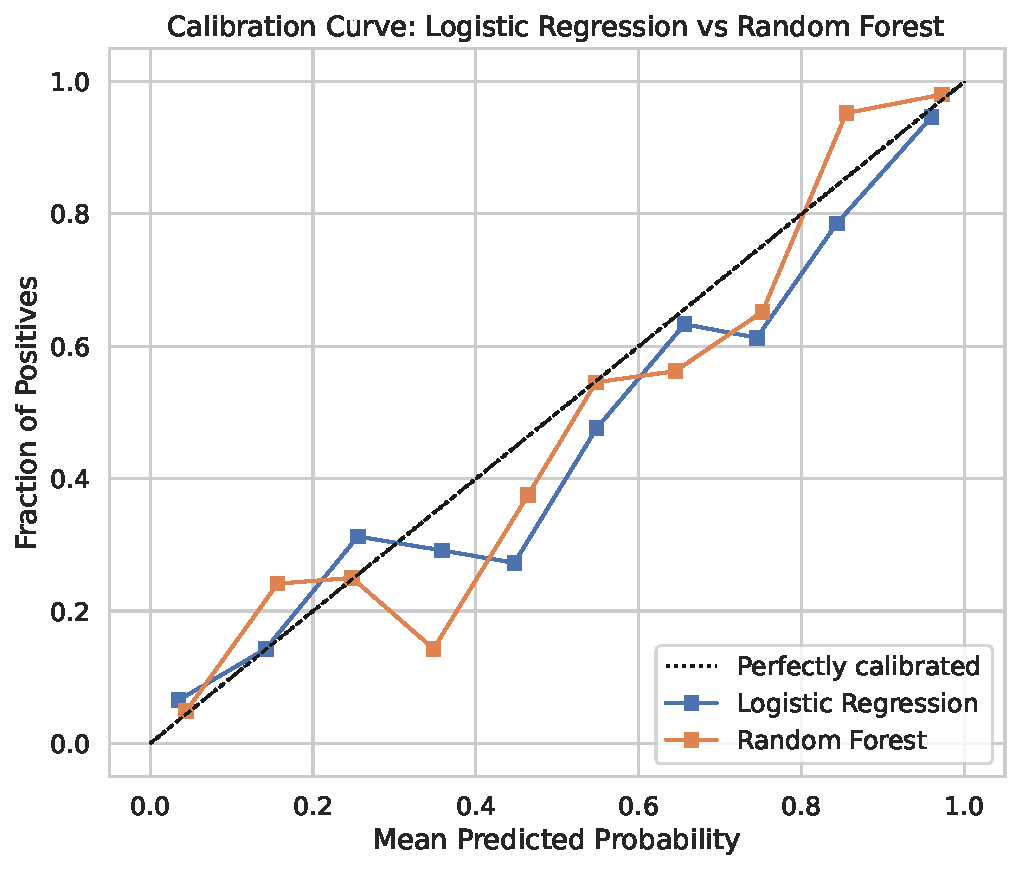
\includegraphics[keepaspectratio]{presentation_files/figure-pdf/cell-15-output-1.pdf}}
\end{center}

\begin{center}\rule{0.5\linewidth}{0.5pt}\end{center}

\subsection{Calibration: Probabilities
vs.~Accuracy}\label{calibration-probabilities-vs.-accuracy-1}

\begin{itemize}
\tightlist
\item
  \textbf{Calibration curve comparison:}

  \begin{itemize}
  \tightlist
  \item
    \textbf{Logistic Regression}

    \begin{itemize}
    \tightlist
    \item
      Follows the 45° line closely → \textbf{strong, smooth
      calibration}.
    \item
      Predicted probabilities align well with observed frequencies.
    \end{itemize}
  \item
    \textbf{Random Forest}

    \begin{itemize}
    \tightlist
    \item
      Also tracks the ideal calibration line with only mild deviations.
    \item
      Slightly less smooth in the mid-range but still \textbf{reasonably
      well calibrated}.
    \end{itemize}
  \end{itemize}
\item
  \textbf{Implication:}

  \begin{itemize}
  \tightlist
  \item
    Both models provide reliable probability estimates, though Logistic
    Regression is \textbf{the most consistently calibrated}.
  \item
    Random Forest delivers slightly better classification accuracy,
    while Logistic Regression is preferred when \textbf{probability
    precision and interpret}
  \end{itemize}
\end{itemize}

\begin{center}\rule{0.5\linewidth}{0.5pt}\end{center}

\subsection{Key Findings}\label{key-findings}

\begin{itemize}
\tightlist
\item
  Higher tuition is associated with higher earnings, but:

  \begin{itemize}
  \tightlist
  \item
    Effects are modest and intertwined with other institutional
    features.
  \end{itemize}
\item
  Retention and completion rates are \textbf{strong, consistent
  predictors} of long-term earnings.
\item
  Institutions with higher \textbf{Pell Grant shares} tend to have lower
  earnings, reflecting underlying socioeconomic differences.
\item
  Model performance:

  \begin{itemize}
  \tightlist
  \item
    Linear and Ridge regression explain \textasciitilde50--57\% of
    earnings variation.
  \item
    Classification models distinguish high- vs low-earning institutions
    with F1 ≈ \textbf{0.77--0.82}.
  \end{itemize}
\item
  Student outcomes and composition matter at least as much as sticker
  price.
\end{itemize}

\begin{center}\rule{0.5\linewidth}{0.5pt}\end{center}

\subsection{Limitations \& Future Work}\label{limitations-future-work}

\begin{itemize}
\tightlist
\item
  \textbf{Data limitations:}

  \begin{itemize}
  \tightlist
  \item
    Institution-level aggregates; no student-level or major-level
    detail.
  \item
    Missing data and reporting differences across institutions.
  \end{itemize}
\item
  \textbf{No causal claims:}

  \begin{itemize}
  \tightlist
  \item
    Observational, cross-sectional analysis; cannot separate institution
    effect from selection bias.
  \end{itemize}
\item
  \textbf{Future directions:}

  \begin{itemize}
  \tightlist
  \item
    Incorporate program/major mix and selectivity.
  \item
    Explore causal methods or matching designs.
  \item
    Examine changes over time (longitudinal trends).
  \end{itemize}
\end{itemize}

\begin{center}\rule{0.5\linewidth}{0.5pt}\end{center}

\subsection{Takeaways}\label{takeaways}

\begin{itemize}
\tightlist
\item
  Tuition alone is an incomplete indicator of value.
\item
  \textbf{Academic success metrics} (retention \& completion) and
  \textbf{student demographics} are central to explaining earnings.
\item
  Machine-learning models provide modest gains in accuracy over linear
  models but highlight similar core drivers.
\item
  For policy, student advising, or institutional benchmarking,
  interpreting \textbf{both cost and outcomes} together is essential.
\end{itemize}




\end{document}
